\documentclass[tikz,border=8pt]{standalone}
\usepackage{lmodern}
\usepackage{amsmath, amssymb}
\usepackage[T1]{fontenc}
\usetikzlibrary{positioning, fit, backgrounds, arrows.meta}

\begin{document}
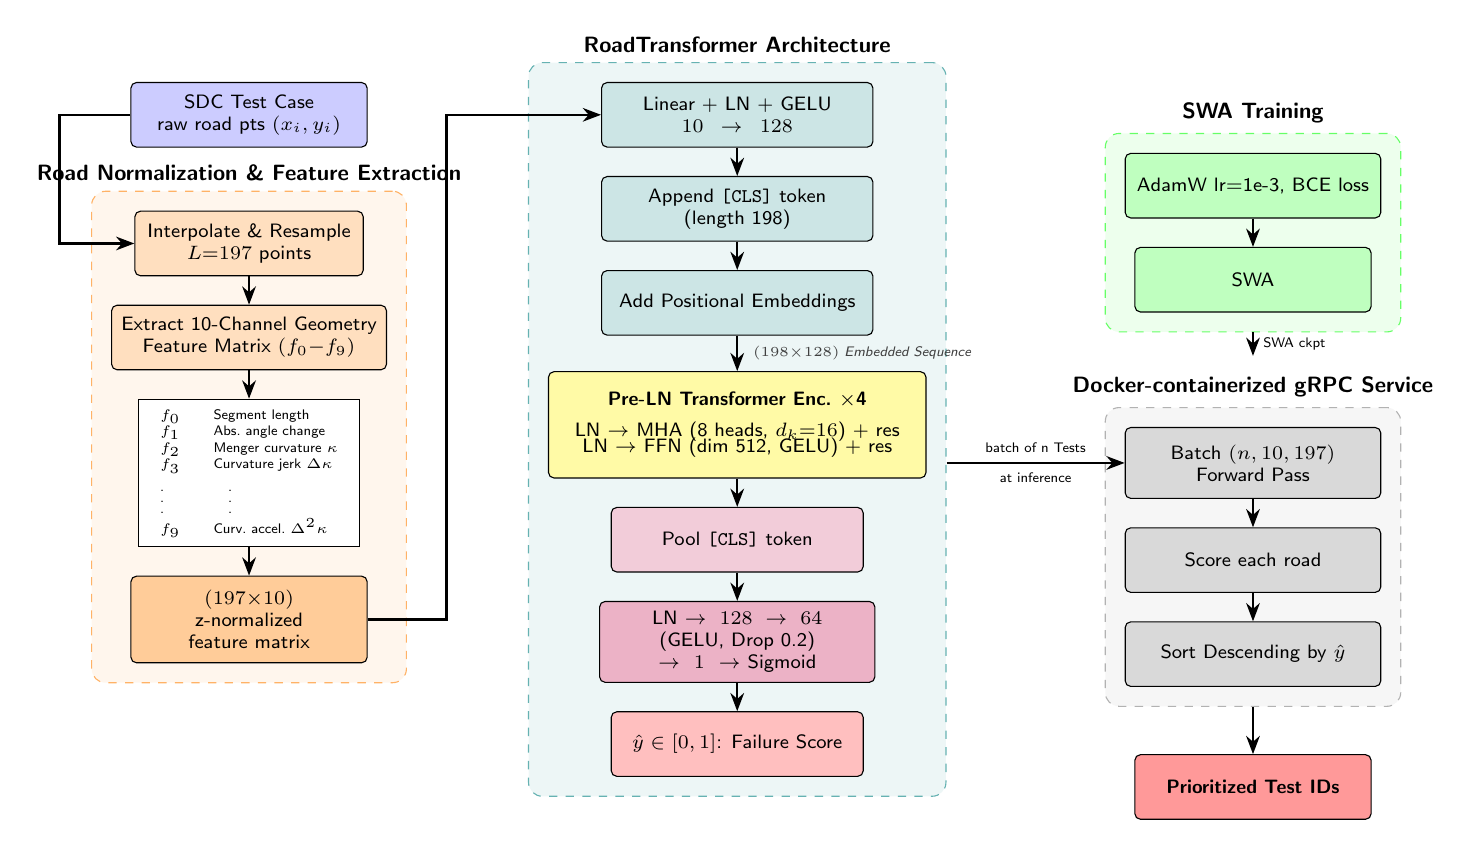
\begin{tikzpicture}[
  font=\sffamily\scriptsize,
  >=Stealth,
  node distance=0.36cm,
  arr/.style={->, thick},
  blk/.style={draw, rounded corners=2pt, fill=#1, align=center,
              inner sep=3.5pt, minimum width=2.9cm, minimum height=0.82cm},
  grp/.style={draw=#1!60, dashed, rounded corners=5pt,
              inner sep=7pt, fill=#1!7},
  htitle/.style={font=\sffamily\bfseries\footnotesize},
]

%% ===== LEFT: INPUT & FEATURE EXTRACTION =====

\node[blk=blue!20, minimum width=3.0cm] (sdc) at (0,0)
    {SDC Test Case\\raw road pts $(x_i, y_i)$};

\node[blk=orange!25, below=0.80cm of sdc] (resamp)
    {Interpolate \& Resample\\$L{=}197$ points};

\node[blk=orange!25, below=0.36cm of resamp] (feat)
    {Extract 10-Channel Geometry\\Feature Matrix $(f_0{-}f_9)$};

\node[draw, fill=white, inner sep=3pt, below=0.36cm of feat,
      font=\sffamily\tiny, minimum width=2.8cm] (ftab)
    {\begin{tabular}{@{}ll@{}}
       $f_0$ & Segment length \\
       $f_1$ & Abs.\ angle change \\
       $f_2$ & Menger curvature $\kappa$ \\
       $f_3$ & Curvature jerk $\Delta\kappa$ \\
       $\vdots$ & \quad $\vdots$ \\
       $f_9$ & Curv.\ accel.\ $\Delta^2\kappa$ \\
     \end{tabular}};

\node[blk=orange!40, below=0.36cm of ftab, minimum width=3.0cm,
      minimum height=1.1cm] (znorm)
    {$(197{\times}10)$\\z-normalized\\feature matrix};

\begin{pgfonlayer}{background}
  \node[grp=orange, fit=(resamp)(feat)(ftab)(znorm),
        label={[htitle]above=2pt:Road Normalization \& Feature Extraction}] (leftgrp) {};
\end{pgfonlayer}

%% ===== MIDDLE: ROADTRANSFORMER ARCHITECTURE =====

\node[blk=teal!20, minimum width=3.2cm, text width=3.2cm] (proj) at (6.2,0)
    {Linear + LN + GELU\\$10 \to 128$};

\node[blk=teal!20, minimum width=3.2cm, text width=3.2cm, below=0.36cm of proj] (cls)
    {Append \texttt{[CLS]} token\\(length 198)};

\node[blk=teal!20, minimum width=3.2cm, text width=3.2cm, below=0.36cm of cls] (posemb)
    {Add Positional Embeddings};

\node[blk=yellow!35, minimum width=3.3cm, minimum height=1.35cm,
      below=0.45cm of posemb] (enc)
    {\begin{tabular}{c}
      \textbf{Pre-LN Transformer Enc.\ $\times$4}\\[3pt]
      {\scriptsize LN $\rightarrow$ MHA (8 heads, $d_k{=}16$) + res}\\[-2pt]
      {\scriptsize LN $\rightarrow$ FFN (dim 512, GELU) + res}
    \end{tabular}};

\node[blk=purple!20, minimum width=3.2cm, below=0.36cm of enc] (pool)
    {Pool \texttt{[CLS]} token};

\node[blk=purple!30, minimum width=3.2cm, text width=3.25cm,
      below=0.36cm of pool, minimum height=0.95cm] (mlp)
    {LN $\to 128 \to 64$\\(GELU, Drop 0.2)\\$\to 1 \to$ Sigmoid};

\node[blk=red!25, minimum width=3.2cm, below=0.36cm of mlp] (yhat)
    {$\hat{y} \in [0,1]$: Failure Score};

\begin{pgfonlayer}{background}
  \node[grp=teal,
        fit=(proj)(cls)(posemb)(enc)(pool)(mlp)(yhat),
        label={[htitle]above:RoadTransformer Architecture}] (midgrp) {};
\end{pgfonlayer}

%% ===== RIGHT: DEPLOYMENT =====

\node[blk=green!25, minimum width=3.0cm, text width=3.0cm] (adam) at (12.75, -0.9)
    {AdamW lr$=$1e-3, BCE loss};

\node[blk=green!25, minimum width=3.0cm, below=0.36cm of adam] (swabox)
    {SWA};

\begin{pgfonlayer}{background}
  \node[grp=green, fit=(adam)(swabox),
        label={[htitle]above:SWA Training}] (swagrp) {};
\end{pgfonlayer}

\node[blk=gray!30, minimum width=3.0cm, text width=3.0cm,
      below=1.20cm of swagrp.south, minimum height=0.90cm] (bfwd)
    {Batch $(n,10,197)$\\Forward Pass};

\node[blk=gray!30, minimum width=3.0cm, text width=3.0cm,
      below=0.36cm of bfwd, minimum height=0.82cm] (scorerd)
    {Score each road};

\node[blk=gray!30, minimum width=3.0cm, text width=3.0cm,
      below=0.36cm of scorerd, minimum height=0.82cm] (sortd)
    {Sort Descending by $\hat{y}$};

\begin{pgfonlayer}{background}
  \node[grp=gray, fit=(bfwd)(scorerd)(sortd),
        label={[htitle]above:Docker-containerized gRPC Service}] (dkgrp) {};
\end{pgfonlayer}

\node[blk=red!40, minimum width=3.0cm, below=0.6cm of dkgrp.south] (result)
    {\textbf{Prioritized Test IDs}};

%% ===== ARROWS =====

\draw[arr] (sdc.west) -- ++(-0.9,0) |- (resamp.west);
\draw[arr] (resamp) -- (feat);
\draw[arr] (feat)   -- (ftab);
\draw[arr] (ftab)   -- (znorm);

\draw[arr] (znorm.east) -- ++(1.00,0) |- (proj.west);

\draw[arr] (proj)   -- (cls);
\draw[arr] (cls)    -- (posemb);
\draw[arr] (posemb) -- node[midway, right=2pt, font=\sffamily\tiny\itshape, text=black!75]
    {$(198{\times}128)$ Embedded Sequence} (enc);
\draw[arr] (enc)    -- (pool);
\draw[arr] (pool)   -- (mlp);
\draw[arr] (mlp)    -- (yhat);

\coordinate (dktitle) at ([yshift=0.65cm]dkgrp.north);
\draw[arr] (adam.south) -- (swabox.north);
\draw[arr] (swagrp.south) -- node[midway, right, font=\sffamily\tiny] {SWA ckpt} (dktitle);
\draw[arr] (bfwd)    -- (scorerd);
\draw[arr] (scorerd) -- (sortd);
\draw[arr] (dkgrp.south) -- (result);

\draw[arr] (midgrp.east |- bfwd.west) -- (bfwd.west)
    node[midway, above, font=\sffamily\tiny] {batch of n Tests}
    node[midway, below, font=\sffamily\tiny] {at inference};

\end{tikzpicture}
\end{document}
